
%% This is a skeleton file demonstrating the use of IEEEtran.cls
%% (requires IEEEtran.cls version 1.7 or later) with an IEEE conference paper.
%%
%% Support sites:
%% http://www.michaelshell.org/tex/ieeetran/
%% http://www.ctan.org/tex-archive/macros/latex/contrib/IEEEtran/
%% and
%% http://www.ieee.org/

%%*************************************************************************
%% Legal Notice:
%% This code is offered as-is without any warranty either expressed or
%% implied; without even the implied warranty of MERCHANTABILITY or
%% FITNESS FOR A PARTICULAR PURPOSE!
%% User assumes all risk.
%% In no event shall IEEE or any contributor to this code be liable for
%% any damages or losses, including, but not limited to, incidental,
%% consequential, or any other damages, resulting from the use or misuse
%% of any information contained here.
%%
%% All comments are the opinions of their respective authors and are not
%% necessarily endorsed by the IEEE.
%%
%% This work is distributed under the LaTeX Project Public License (LPPL)
%% ( http://www.latex-project.org/ ) version 1.3, and may be freely used,
%% distributed and modified. A copy of the LPPL, version 1.3, is included
%% in the base LaTeX documentation of all distributions of LaTeX released
%% 2003/12/01 or later.
%% Retain all contribution notices and credits.
%% ** Modified files should be clearly indicated as such, including  **
%% ** renaming them and changing author support contact information. **
%%
%% File list of work: IEEEtran.cls, IEEEtran_HOWTO.pdf, bare_adv.tex,
%%                    bare_conf.tex, bare_jrnl.tex, bare_jrnl_compsoc.tex
%%*************************************************************************

% *** Authors should verify (and, if needed, correct) their LaTeX system  ***
% *** with the testflow diagnostic prior to trusting their LaTeX platform ***
% *** with production work. IEEE's font choices can trigger bugs that do  ***
% *** not appear when using other class files.                            ***
% The testflow support page is at:
% http://www.michaelshell.org/tex/testflow/



% Note that the a4paper option is mainly intended so that authors in
% countries using A4 can easily print to A4 and see how their papers will
% look in print - the typesetting of the document will not typically be
% affected with changes in paper size (but the bottom and side margins will).
% Use the testflow package mentioned above to verify correct handling of
% both paper sizes by the user's LaTeX system.
%
% Also note that the "draftcls" or "draftclsnofoot", not "draft", option
% should be used if it is desired that the figures are to be displayed in
% draft mode.
%
\documentclass[conference]{IEEEtran}
% Add the compsoc option for Computer Society conferences.
%
% If IEEEtran.cls has not been installed into the LaTeX system files,
% manually specify the path to it like:
% \documentclass[conference]{../sty/IEEEtran}





% Some very useful LaTeX packages include:
% (uncomment the ones you want to load)


% *** MISC UTILITY PACKAGES ***
%
%\usepackage{ifpdf}
% Heiko Oberdiek's ifpdf.sty is very useful if you need conditional
% compilation based on whether the output is pdf or dvi.
% usage:
% \ifpdf
%   % pdf code
% \else
%   % dvi code
% \fi
% The latest version of ifpdf.sty can be obtained from:
% http://www.ctan.org/tex-archive/macros/latex/contrib/oberdiek/
% Also, note that IEEEtran.cls V1.7 and later provides a builtin
% \ifCLASSINFOpdf conditional that works the same way.
% When switching from latex to pdflatex and vice-versa, the compiler may
% have to be run twice to clear warning/error messages.






% *** CITATION PACKAGES ***
%
%\usepackage{cite}
% cite.sty was written by Donald Arseneau
% V1.6 and later of IEEEtran pre-defines the format of the cite.sty package
% \cite{} output to follow that of IEEE. Loading the cite package will
% result in citation numbers being automatically sorted and properly
% "compressed/ranged". e.g., [1], [9], [2], [7], [5], [6] without using
% cite.sty will become [1], [2], [5]--[7], [9] using cite.sty. cite.sty's
% \cite will automatically add leading space, if needed. Use cite.sty's
% noadjust option (cite.sty V3.8 and later) if you want to turn this off.
% cite.sty is already installed on most LaTeX systems. Be sure and use
% version 4.0 (2003-05-27) and later if using hyperref.sty. cite.sty does
% not currently provide for hyperlinked citations.
% The latest version can be obtained at:
% http://www.ctan.org/tex-archive/macros/latex/contrib/cite/
% The documentation is contained in the cite.sty file itself.






% *** GRAPHICS RELATED PACKAGES ***
%
\ifCLASSINFOpdf
  % \usepackage[pdftex]{graphicx}
  % declare the path(s) where your graphic files are
  % \graphicspath{{../pdf/}{../jpeg/}}
  % and their extensions so you won't have to specify these with
  % every instance of \includegraphics
  % \DeclareGraphicsExtensions{.pdf,.jpeg,.png}
\else
  % or other class option (dvipsone, dvipdf, if not using dvips). graphicx
  % will default to the driver specified in the system graphics.cfg if no
  % driver is specified.
  % \usepackage[dvips]{graphicx}
  % declare the path(s) where your graphic files are
  % \graphicspath{{../eps/}}
  % and their extensions so you won't have to specify these with
  % every instance of \includegraphics
  % \DeclareGraphicsExtensions{.eps}
\fi
% graphicx was written by David Carlisle and Sebastian Rahtz. It is
% required if you want graphics, photos, etc. graphicx.sty is already
% installed on most LaTeX systems. The latest version and documentation can
% be obtained at:
% http://www.ctan.org/tex-archive/macros/latex/required/graphics/
% Another good source of documentation is "Using Imported Graphics in
% LaTeX2e" by Keith Reckdahl which can be found as epslatex.ps or
% epslatex.pdf at: http://www.ctan.org/tex-archive/info/
%
% latex, and pdflatex in dvi mode, support graphics in encapsulated
% postscript (.eps) format. pdflatex in pdf mode supports graphics
% in .pdf, .jpeg, .png and .mps (metapost) formats. Users should ensure
% that all non-photo figures use a vector format (.eps, .pdf, .mps) and
% not a bitmapped formats (.jpeg, .png). IEEE frowns on bitmapped formats
% which can result in "jaggedy"/blurry rendering of lines and letters as
% well as large increases in file sizes.
%
% You can find documentation about the pdfTeX application at:
% http://www.tug.org/applications/pdftex

\usepackage{graphicx}
\usepackage{amssymb}
\usepackage{leqno}
\usepackage{cases}

% *** MATH PACKAGES ***
%
\usepackage[cmex10]{amsmath}
% A popular package from the American Mathematical Society that provides
% many useful and powerful commands for dealing with mathematics. If using
% it, be sure to load this package with the cmex10 option to ensure that
% only type 1 fonts will utilized at all point sizes. Without this option,
% it is possible that some math symbols, particularly those within
% footnotes, will be rendered in bitmap form which will result in a
% document that can not be IEEE Xplore compliant!
%
% Also, note that the amsmath package sets \interdisplaylinepenalty to 10000
% thus preventing page breaks from occurring within multiline equations. Use:
%\interdisplaylinepenalty=2500
% after loading amsmath to restore such page breaks as IEEEtran.cls normally
% does. amsmath.sty is already installed on most LaTeX systems. The latest
% version and documentation can be obtained at:
% http://www.ctan.org/tex-archive/macros/latex/required/amslatex/math/


\usepackage{amsthm}


% *** SPECIALIZED LIST PACKAGES ***
%
%\usepackage{algorithmic}
% algorithmic.sty was written by Peter Williams and Rogerio Brito.
% This package provides an algorithmic environment fo describing algorithms.
% You can use the algorithmic environment in-text or within a figure
% environment to provide for a floating algorithm. Do NOT use the algorithm
% floating environment provided by algorithm.sty (by the same authors) or
% algorithm2e.sty (by Christophe Fiorio) as IEEE does not use dedicated
% algorithm float types and packages that provide these will not provide
% correct IEEE style captions. The latest version and documentation of
% algorithmic.sty can be obtained at:
% http://www.ctan.org/tex-archive/macros/latex/contrib/algorithms/
% There is also a support site at:
% http://algorithms.berlios.de/index.html
% Also of interest may be the (relatively newer and more customizable)
% algorithmicx.sty package by Szasz Janos:
% http://www.ctan.org/tex-archive/macros/latex/contrib/algorithmicx/




% *** casesMENT PACKAGES ***
%
%\usepackage{array}
% Frank Mittelbach's and David Carlisle's array.sty patches and improves
% the standard LaTeX2e array and tabular environments to provide better
% appearance and additional user controls. As the default LaTeX2e table
% generation code is lacking to the point of almost being broken with
% respect to the quality of the end results, all users are strongly
% advised to use an enhanced (at the very least that provided by array.sty)
% set of table tools. array.sty is already installed on most systems. The
% latest version and documentation can be obtained at:
% http://www.ctan.org/tex-archive/macros/latex/required/tools/


%\usepackage{mdwmath}
%\usepackage{mdwtab}
% Also highly recommended is Mark Wooding's extremely powerful MDW tools,
% especially mdwmath.sty and mdwtab.sty which are used to format equations
% and tables, respectively. The MDWtools set is already installed on most
% LaTeX systems. The lastest version and documentation is available at:
% http://www.ctan.org/tex-archive/macros/latex/contrib/mdwtools/


% IEEEtran contains the IEEEeqnarray family of commands that can be used to
% generate multiline equations as well as matrices, tables, etc., of high
% quality.


%\usepackage{eqparbox}
% Also of notable interest is Scott Pakin's eqparbox package for creating
% (automatically sized) equal width boxes - aka "natural width parboxes".
% Available at:
% http://www.ctan.org/tex-archive/macros/latex/contrib/eqparbox/





% *** SUBFIGURE PACKAGES ***
%\usepackage[tight,footnotesize]{subfigure}
% subfigure.sty was written by Steven Douglas Cochran. This package makes it
% easy to put subfigures in your figures. e.g., "Figure 1a and 1b". For IEEE
% work, it is a good idea to load it with the tight package option to reduce
% the amount of white space around the subfigures. subfigure.sty is already
% installed on most LaTeX systems. The latest version and documentation can
% be obtained at:
% http://www.ctan.org/tex-archive/obsolete/macros/latex/contrib/subfigure/
% subfigure.sty has been superceeded by subfig.sty.



%\usepackage[caption=false]{caption}
%\usepackage[font=footnotesize]{subfig}
% subfig.sty, also written by Steven Douglas Cochran, is the modern
% replacement for subfigure.sty. However, subfig.sty requires and
% automatically loads Axel Sommerfeldt's caption.sty which will override
% IEEEtran.cls handling of captions and this will result in nonIEEE style
% figure/table captions. To prevent this problem, be sure and preload
% caption.sty with its "caption=false" package option. This is will preserve
% IEEEtran.cls handing of captions. Version 1.3 (2005/06/28) and later
% (recommended due to many improvements over 1.2) of subfig.sty supports
% the caption=false option directly:
%\usepackage[caption=false,font=footnotesize]{subfig}
%
% The latest version and documentation can be obtained at:
% http://www.ctan.org/tex-archive/macros/latex/contrib/subfig/
% The latest version and documentation of caption.sty can be obtained at:
% http://www.ctan.org/tex-archive/macros/latex/contrib/caption/




% *** FLOAT PACKAGES ***
%
%\usepackage{fixltx2e}
% fixltx2e, the successor to the earlier fix2col.sty, was written by
% Frank Mittelbach and David Carlisle. This package corrects a few problems
% in the LaTeX2e kernel, the most notable of which is that in current
% LaTeX2e releases, the ordering of single and double column floats is not
% guaranteed to be preserved. Thus, an unpatched LaTeX2e can allow a
% single column figure to be placed prior to an earlier double column
% figure. The latest version and documentation can be found at:
% http://www.ctan.org/tex-archive/macros/latex/base/



%\usepackage{stfloats}
% stfloats.sty was written by Sigitas Tolusis. This package gives LaTeX2e
% the ability to do double column floats at the bottom of the page as well
% as the top. (e.g., "\begin{figure*}[!b]" is not normally possible in
% LaTeX2e). It also provides a command:
%\fnbelowfloat
% to enable the placement of footnotes below bottom floats (the standard
% LaTeX2e kernel puts them above bottom floats). This is an invasive package
% which rewrites many portions of the LaTeX2e float routines. It may not work
% with other packages that modify the LaTeX2e float routines. The latest
% version and documentation can be obtained at:
% http://www.ctan.org/tex-archive/macros/latex/contrib/sttools/
% Documentation is contained in the stfloats.sty comments as well as in the
% presfull.pdf file. Do not use the stfloats baselinefloat ability as IEEE
% does not allow \baselineskip to stretch. Authors submitting work to the
% IEEE should note that IEEE rarely uses double column equations and
% that authors should try to avoid such use. Do not be tempted to use the
% cuted.sty or midfloat.sty packages (also by Sigitas Tolusis) as IEEE does
% not format its papers in such ways.





% *** PDF, URL AND HYPERLINK PACKAGES ***
%
%\usepackage{url}
% url.sty was written by Donald Arseneau. It provides better support for
% handling and breaking URLs. url.sty is already installed on most LaTeX
% systems. The latest version can be obtained at:
% http://www.ctan.org/tex-archive/macros/latex/contrib/misc/
% Read the url.sty source comments for usage information. Basically,
% \url{my_url_here}.





% *** Do not adjust lengths that control margins, column widths, etc. ***
% *** Do not use packages that alter fonts (such as pslatex).         ***
% There should be no need to do such things with IEEEtran.cls V1.6 and later.
% (Unless specifically asked to do so by the journal or conference you plan
% to submit to, of course. )


% correct bad hyphenation here
%\hyphenation{op-tical net-works semi-conduc-tor}


\begin{document}
%
% paper title
% can use linebreaks \\ within to get better formatting as desired
\title{Sequential Verification over Galois Field based on Word-level Abstraction}


% author names and affiliations
% use a multiple column layout for up to three different
% affiliations
\author{
\IEEEauthorblockN{Xiaojun Sun}
\IEEEauthorblockA{Electrical and Computer Engineering\\
University of Utah\\
Salt Lake City, Utah\\
Email: xiaojun.sun@utah.edu}
\and
\IEEEauthorblockN{Priyank Kalla}
\IEEEauthorblockA{Electrical and Computer Engineering\\
University of Utah\\
Salt Lake City, Utah\\
Email: kalla@ece.utah.edu}

}

% conference papers do not typically use \thanks and this command
% is locked out in conference mode. If really needed, such as for
% the acknowledgment of grants, issue a \IEEEoverridecommandlockouts
% after \documentclass

% for over three affiliations, or if they all won't fit within the width
% of the page, use this alternative format:
%
%\author{\IEEEauthorblockN{Michael Shell\IEEEauthorrefmark{1},
%Homer Simpson\IEEEauthorrefmark{2},
%James Kirk\IEEEauthorrefmark{3},
%Montgomery Scott\IEEEauthorrefmark{3} and
%Eldon Tyrell\IEEEauthorrefmark{4}}
%\IEEEauthorblockA{\IEEEauthorrefmark{1}School of Electrical and Computer Engineering\\
%Georgia Institute of Technology,
%Atlanta, Georgia 30332--0250\\ Email: see http://www.michaelshell.org/contact.html}
%\IEEEauthorblockA{\IEEEauthorrefmark{2}Twentieth Century Fox, Springfield, USA\\
%Email: homer@thesimpsons.com}
%\IEEEauthorblockA{\IEEEauthorrefmark{3}Starfleet Academy, San Francisco, California 96678-2391\\
%Telephone: (800) 555--1212, Fax: (888) 555--1212}
%\IEEEauthorblockA{\IEEEauthorrefmark{4}Tyrell Inc., 123 Replicant Street, Los Angeles, California 90210--4321}}




% use for special paper notices
%\IEEEspecialpapernotice{(Invited Paper)}




% make the title area
\maketitle


%\begin{abstract}
%%\boldmath
%The abstract goes here.
%\end{abstract}
% IEEEtran.cls defaults to using nonbold math in the Abstract.
% This preserves the distinction between vectors and scalars. However,
% if the conference you are submitting to favors bold math in the abstract,
% then you can use LaTeX's standard command \boldmath at the very start
% of the abstract to achieve this. Many IEEE journals/conferences frown on
% math in the abstract anyway.

% no keywords




% For peer review papers, you can put extra information on the cover
% page as needed:
% \ifCLASSOPTIONpeerreview
% \begin{center} \bfseries EDICS Category: 3-BBND \end{center}
% \fi
%
% For peerreview papers, this IEEEtran command inserts a page break and
% creates the second title. It will be ignored for other modes.
\IEEEpeerreviewmaketitle

\begin{abstract}
%\boldmath
This paper introduce a method to apply \emph{Word-level Abstraction} to sequential arithmetic circuits verification.
Details of word-level abstraction are concluded in Tim's IWLS and FMCAD paper. Here we discuss more on 
Sequential Multiplier with Parallel Output (SMPO) designed for normal basis multiplication, as well as \emph{optimal 
normal basis theory}.
\end{abstract}


\section{Fundamentals on Mathematics}
	\subsection{Normal Basis Theory}
Let $\beta$ be a element in the Galois field $F_{2^n}$ constructed by primitive element $\alpha$ and minimal polynomial 
$f(\alpha)$. Then a basis in the form $\{\beta, \beta^2, \beta^4, \beta^8, ... ,\beta^{2^{n-1}}\}$ is a
\emph{Normal Basis}; here $\beta$ is called \emph{Normal Element}.\\

All about normal basis theory can be found in \textit{Gao's Thesis}. \cite{Gao}

	\subsection{Normal Basis Multiplication}
For arithmetic in Galois fields, multiplication (with modulus) can be greatly simplified if Normal Basis representation 
is adopted to represent operands, especially in element square and multiplication:\\

\textit{Example 1:}\ \ Element square: In $F_{2^n}$, we have relation $(a+b)^2 = a^2 + b^2$. Then 
$(b_0\beta + b_1\beta^2 + b_2\beta^4 + \dots + b_{n-1}\beta^{2^{n-1}})^2 = 
b_0^2\beta^2 + b_1^2\beta^4 + b_2^2\beta^8 + \dots + b_{n-1}^2\beta = 
b_{n-1}^2\beta + b_0\beta^2 + b_1\beta^4 + \dots + b_{n-2}\beta^{2^{n-1}}$, which means a simple right-cyclic rotation.
One the other hand, standard basis representation do not have this benefit:\\
In $F_{2^3}$ constructed by $\alpha^3 + \alpha + 1$, standard basis is $\{ 1, \alpha, \alpha^2\}$.
Let $\beta = \alpha^3$, $N = \{ \beta, \beta^2, \beta^4\}$ is a normal basis. Write down an element with both representations:
$E = a_0 + a_1\alpha + a_2\alpha^2 = b_0\beta + b_1\beta^2 + b_2\beta^4$, and its square in standard basis:
$E^2 = a_0 + a_1\alpha^2 + a_2\alpha^4 = a_0 + a_2\alpha + (a_1 + a_2)\alpha^2$. When it is written in normal basis:
$E^2 = b_2\beta + b_0\beta^2 + b_1\beta^4$, no additional terms, just simple rotation.\\

\textit{Example 2:}\ \ Normal basis multiplication: Suppose we have 2 binary vectors representing 2 operands in normal
basis: $A = (a_0, a_1, \dots, a_{n-1}), B = (b_0, b_1, \dots, b_{n-1})$; similarly the product can also be written
as: $C = A*B = (c_0, c_1, \dots, c_{n-1}).$\\
Then the highest digit of product can be got with some function: $c_{n-1} = f(a_0, a_1, \dots, a_{n-1}; b_0, b_1, 
\dots, b_{n-1})$. Square both side: $C^2 = A^2*B^2$, i.e. the second highest digit $c_{n-2} = f(a_{n-1}, a_0, a_1, 
\dots, a_{n-2}; b_{n-1}, b_0, b_1, \dots, b_{n-2}).$ By this method it is easy to get all digits of product $C$.\\

\textit{Example 3:}\ \ $\lambda$-Matrix: We can use a binary $n\times n$ matrix $M$ to describe the "function"
 mentioned above: $c_{n-1} = f(A, B) = A \cdot M \cdot B^T$, $B^T$ denotes vector transposition. 
More specifically, we can denote the matrix by \emph{$k$-th $\lambda$-Matrix}: $c_k = A \cdot M^{(k)} \cdot B^T$.
Then $c_{k-1} = A \cdot M^{(k-1)} \cdot B^T = rotate(A) \cdot M^{(k)} \cdot rotate(B)^T$, which means
by right and down shifting $M^{(k-1)}$ we can get $M^{(k)}$.\\
In $F_{2^3}$ constructed by $\alpha^3 + \alpha + 1$, let $\beta = \alpha^3$, $N = \{ \beta, \beta^2, \beta^4\}$ 
is a normal basis. $0$-th $\lambda$-Matrix
\begin{equation}
M^{(0)} = \left(
\begin{array} {lcr}
0 & 1 & 0\\
1 & 0 & 1\\
0 & 1 & 1
\end{array} \right).
\end{equation}
i.e.,
\begin{equation}
c_0 = (a_0\  a_1\  a_2)\left(
\begin{array} {lcr}
0 & 1 & 0\\
1 & 0 & 1\\
0 & 1 & 1
\end{array} \right)\left(
\begin{array} {lcr}
b_0\\
b_1\\
b_2
\end{array} \right).
\end{equation}

\indent \\
$\lambda$-Matrix is defined with cross-product terms from multiplication. That is 
\begin{equation}
Product C = (\sum_{i=0}^{n-1}a_i\beta^{2^i})(\sum_{j=0}^{n-1}b_j\beta^{2^j}) = \sum_{i=0}^{n-1}\sum_{j=0}^{n-1}a_ib_j\beta^{2^i}\beta^{2^j}
\end{equation}
The expressions $\beta^{2^i}\beta^{2^j}$ are referred to as cross-product terms, and can be represented by
normal basis, i.e.
\begin{equation}
\beta^{2^i}\beta^{2^j} = \sum_{k=0}^{n-1}\lambda_{ij}^{(k)}\beta^{2^k}, \ \ \lambda_{ij}^{(k)} \in F_2.
\end{equation}
Substitution yields, get the expression for k-th digit of product as showed in \textit{Example 3}:
\begin{equation}
c_k = \sum_{i=0}^{n-1}\sum_{j=0}^{n-1}\lambda_{ij}^{(k)}a_ib_j
\end{equation}
$\lambda_{ij}^{(k)}$ is the entry with coordinate $(i,j)$ in $k$-th $\lambda$-Matrix.\par
From examples above we can see the advantages of using normal basis representation. Then how can we find out
normal element based on primitive element? Meanwhile, how to compute $\lambda$-Matrix? In the following part
we will figure out a kind of normal basis with specific properties, which will make $\lambda$-Matrix easy to calculate.


%Noticed the difference between matrix in multiplication and official-defined multiplication table? Please refer
%to the Problem part in \textit{ref1: write-up about normal basis}.

\section{Optimal Normal Basis}
	\subsection{Complexity \& ONB Definition}
%%$\lambda$-Matrix varies with different digit of result vector, so sometimes a normal-basis-determined matrix
%%needs to be defined, that is \emph{Multiplication Table}. The definition of multiplication table $T$ is here:
%%\begin{equation}
%%\beta \left( \begin{array} {lcr}
%% \beta \\ 
%%\beta^2 \\ 
%%\cdot \\ 
%%\cdot \\ 
%%\cdot \\ 
%%\beta^{2^{n-1}} 
%%\end{array} \right) = T \left( \begin{array} {lcr}
%% \beta \\ 
%%\beta^2 \\ 
%%\cdot \\ 
%%\cdot \\ 
%%\cdot \\ 
%%\beta^{2^{n-1}} 
%%\end{array} \right)
%%\end{equation}
The number of non-zero entries in $\lambda$-Matrix is known as  \emph{Complexity$(C_N)$}. \\
To define optimal normal basis, it is necessary to find out the minimum number
of non-zero terms in $\lambda$-matrix.\\
\textit{Theorem}\ \ If N is a normal basis for $F_{p^n}$ with $\lambda$-matrix $M^{(k)}$, then non-zero entries in 
matrix $C_N\geq 2n-1$.\\
\begin{proof}
Let $N = \{\beta, \beta^p, \beta^{p^2},\dots, \beta^{p^{n-1}}\}$, denote $\beta^{p^i}$ by $\beta_i$. 
Then $\sum_{i=0}^{n-1} \beta_i = trace\ \beta$. \\
Denote $trace\ \beta$ with $b$, consider $n\times n$ matrix $M^{(0)}$. Then\\
$b\beta_0 = \sum_{i=0}^{n-1} \beta \beta_i$.\\
Therefore, the sum of all rows in $M^{(0)}$ is an n-tuple with $b$ as the first element and zeros elsewhere.
So the first column must contain at least 1 nonzero element, and other columns must get a sum of zero 
while keeping every row linearly independent so there should be at least 2 non-zero elements each column.
\end{proof}
If there exists a set of normal basis satisfying $C_N = 2n - 1$, this normal basis is named as
\emph{Optimal Normal Basis}.\\
%For $F_{2^n}$, easy to figure out the first row of multiplication table must contain one "1" because 
%$\beta \beta^{2^0} = \beta^{2^1}$. for the rest rows $\beta \beta^{2^i} \neq \beta^{2^{i+1}}$,
%so there must be at least 2 "1"s to fulfil the equation. So for multiplication table, $C_N\geq 2n-1$ also holds.\\

\textit{Example 4:}\ \ In $F_{2^4}$ constructed with $\alpha^4 + \alpha + 1$, 2 sets of normal basis can be found:
$\beta = \alpha^3, N = \{ \alpha^3, \alpha^6, \alpha^{12}, \alpha^9\}$ and 
$\beta = \alpha^7, N = \{\alpha^7, \alpha^{14}, \alpha^{13}, \alpha^{11}\}$. Multiplication table for $\beta = \alpha^3$:
\begin{equation}
T_1 = \left(
\begin{array}{lccr}
0 & 1 & 0 & 0\\
0 & 0 & 0 & 1\\
1 & 1 & 1 & 1\\
0 & 0 & 1 & 0
\end{array} \right)
\end{equation}
Complexity $C_N$ = 7, this is optimal. For $\beta = \alpha^7$:
\begin{equation}
T_2 = \left(
\begin{array}{lccr}
0 & 1 & 0 & 0\\
1 & 1 & 0 & 1\\
1 & 0 & 1 & 0\\
1 & 0 & 1 & 1
\end{array} \right)
\end{equation}
Complexity $C_N$ = 9, this is NOT optimal.\\

There should be an efficient method to construct optimal normal basis. Following contents mainly come from refernce book\cite{ECC}.

	\subsection{Type-I Optimal Normal Basis}
Rules for creating Type-I ONB over $F_{2^n}$ are:
\begin{itemize}
\item n+1 must be prime.
\item 2 must be primitive in $\mathbb{Z}_{n+1}$.
\end{itemize}
Second rule means 2 raise to any power 0 $\sim$ n-1 (mod n+1) must cover every integer 1 $\sim$ n.\\
$\lambda_{ij}^{(k)}$ is the entry with coordinate $(i,j)$ from k-th $\lambda$-Matrix. Then the crossproduct
term can be written as
\begin{equation}
\beta^{2^i}\beta^{2^j} = \sum_{k=0}^{n-1} \lambda_{ij}^{(k)} \beta^{2^k}
\end{equation}
Suppose we only care about k=0. So simplified to following equations:
\begin{numcases}{}
\beta^{2^i}\beta^{2^j} = \beta\\
\beta^{2^i}\beta^{2^j} = 1 \ \ (if\ \  2^i \equiv 2^j\ \  mod\ \  n+1)
\end{numcases}
solution $(i,j)$ implies entries equal to "1" in matrix. If $\beta$ is already an optimal normal element, 
$\beta^{2^i}$ counts through all powers of $\beta$ and generates our basis. So
\begin{numcases}{}
2^i + 2^j = 1 \ \ mod\ \  n+1\\
2^i + 2^j = 0 \ \ mod \ \ n+1
\end{numcases}
have the same solution for $M^{(0)}$. Note this method can be applied even both primitive polynomial and normal element are unkown (but existance and adoption of optimal normal basis must be guaranteed).\\
If do similar thing, equations for multiplication table can also be obtained. Based on this, a transformation relation 
between $\lambda$-Matrix and Multiplication table can be concluded. However, the proof is still a \textbf{problem}.
\textit{BTW, example 4 shows a type-I ONB over $F_{2^4}$}.


	\subsection{Type-II Optimal Normal Basis}
Rules for creating Type-II ONB over $F_{2^n}$ are:
\begin{itemize}
\item 2n+1 must be prime. And either
\item 2 must be primitive in $\mathbb{Z}_{2n+1}$, OR
\item $2n+1 \equiv 3 \ \ mod\ \  4$ AND 2 generates the quadratic residues in $\mathbb{Z}_{2n+1}$
\end{itemize}
The last rule means: The last 2 bits are set in the binary representation of prime 2n+1; even if $2^k \ \ mod\ \  2n+1$ does not
generate every element in 0 $\sim$ 2n, we can at least take the square root $mod\ \  2n+1$ of $2^k$. (Need to learn more on quadratic residues)\\
To generate a Type-II ONB, pick an element $\gamma$ of order 2n+1 in $F_{2^{2n}}$, then use this to find optimal normal 
element from $F_{2^n}$: $\beta = \gamma + \gamma^{-1}$. Crossproduct terms
\begin{equation}
\begin{split}
\beta^{2^i}\beta^{2^j} &= (\gamma^{2^i} + \gamma^{-2^i})(\gamma^{2^j} + \gamma^{-2^j})\\ &= 
(\gamma^{2^i+2^j} + \gamma^{-(2^i+2^j)}) + (\gamma^{2^i-2^j} + \gamma^{-(2^i-2^j)})\\ &= 
\begin{cases}
\beta^{2^k} + \beta^{2^{k\prime}}\ \  if\ 2^i \neq 2^j \ \ mod\ \  2n+1\\
\beta^{2^k}\ \  if\ 2^i \equiv 2^j \ \ mod\ \  2n+1
\end{cases}
\end{split}
\end{equation}
$k$ and $k\prime$ are the 2 possible solutions to multiplication of any 2 basis elements. That's what makes this normal basis
optimal: it has the minimum number of possible terms. In the case of $2^i \neq 2^j \ \ mod\ \  2n+1$, at least one of these
equations:
\begin{equation}
\begin{cases}
2^i + 2^j = 2^k \ \ mod\ \  2n+1\\
2^i + 2^j = -2^k \ \ mod \ \ 2n+1
\end{cases}
\end{equation}
will have a solution, and at least one of these equations:
\begin{equation}
\begin{cases}
2^i - 2^j = 2^{k\prime} \ \ mod \ \ 2n+1\\
2^i - 2^j = -2^{k\prime} \ \ mod \ \ 2n+1
\end{cases}
\end{equation}
also has a solution.\\
In the case of $2^i \equiv \pm 2^j \ \ mod\ \  2n+1$, at least one of the following 4 equations has a solution:
\begin{equation}
\begin{cases}
2^i + 2^j = 2^k \ \ mod \ \ 2n+1\\
2^i + 2^j = -2^k \ \ mod \ \ 2n+1\\
2^i - 2^j = 2^k \ \ mod\ \  2n+1\\
2^i - 2^j = -2^k \ \ mod \ \ 2n+1
\end{cases}
\end{equation}
In the first set of equations, there are two possible solutions, and in the second set of equations,
there is only one possible solution. It is easy to see that the equations are all similar, so instead of 
working with 2 different sets we can combine them and work with just one group of 4 equations. To build 
our $\lambda$-Matrix, we set k=0 and find solutions to:
\begin{equation}
\begin{cases}
2^i + 2^j = 1 \ \mod\ \  2n+1\\
2^i + 2^j = -1 \ \ mod \ \ 2n+1\\
2^i - 2^j = 1 \ \ mod\ \  2n+1\\
2^i - 2^j = -1 \ \ mod \ \ 2n+1
\end{cases}
\end{equation}

\textit{Example 5:} \ \ Following this criteria, easy to find $M^{(0)}$ for $F_{2^5}$:
\begin{equation}
M^{(0)} = \left(
\begin{array}{lcccr}
0 & 1 & 0 & 0 & 0\\
1 & 0 & 0 & 1 & 0\\
0 & 0 & 0 & 1 & 1\\
0 & 1 & 1 & 0 & 0\\
0 & 0 & 1 & 0 & 1
\end{array} \right)
\end{equation}


More details about proof can be found in \cite{ONB}, which is believed to be first paper on ONB theory.\\
Now from the simplified criteria we get, it is not expensive any more to compute a $\lambda$-Matrix.
Moreover, one advantage adopting this criteria is that for multiplier designers, they can design without knowing
specific normal element (althought this optimal normal element is unique when primitive polynomial is set).
However, for our approach it is necessary to find out what optimal normal element we are using.
So the problem is: If field extension and primitive polynomial ($F_{2^n}$ and $f(\alpha)$) is given, and
we already get the $\lambda$-Matrix (which means we know a type I or II optimal normal basis is adopted), is it 
possible to find an efficient way to compute corresponding optimal normal element?


\section{Normal Basis Multiplier}
	\subsection{SMPO Design}
This part mainly comes from \textit{ref2:SMPO}. \cite{SMPO}\\
Based on the normal basis multiplication in Example 2, Massey and Omura designed a Sequential Multiplier with Serial
Output, get every bit of output by shifting operands 1 bit per clock.
\begin{figure}
\centering
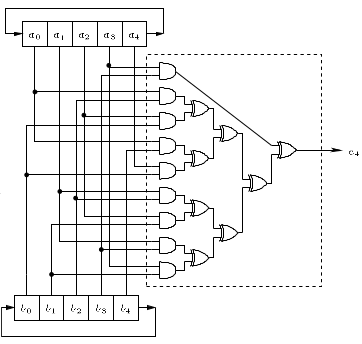
\includegraphics[width=2.5in]{SMSO.png}
\caption{Massey-Omura SMSO for m-bit}
\label{fig_SMSO}
\end{figure}

For 5-bit SMSO, based on $\lambda$-Matrix we got from \textit{Example 5}, consider following equation \\
$c_i = b_ia_{i+1} + b_{i+1}(a_i + a_{i+3}) + b_{i+2}(a_{i+3} + a_{i+4}) + b_{i+3}(a_{i+1} + a_{i+2}) + b_{i+4}
(a_{i+2} + a_{i+4}), 0\leq i\leq 4$\\
It is possible to calculate every product term within one clock. Also utilize cyclic similarity, we have SMPO
design:
\begin{figure}
\centering
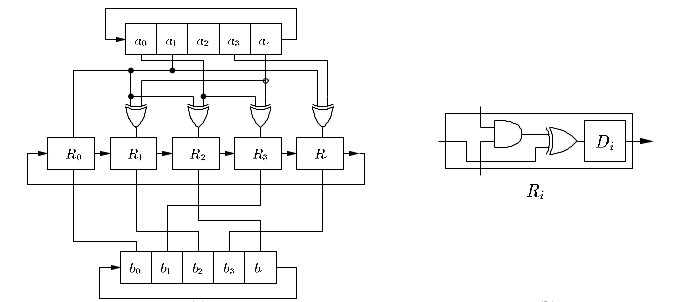
\includegraphics[width=2.5in]{SMPO.png}
\caption{5-bit SMPO design}
\label{fig_SMPO}
\end{figure}

\textit{Example 6:}\ \ Sequential Multiplier Protocol:
\begin{itemize}
\item \textbf{Initial}\ \ $R_0 = R_1 = R_2 = R_3 = R_4 = 0$
\item \textbf{Clock 1}\ \ $R_0 = a_1b_0, R_1 = b_2(a_1 + a_4), R_2 = b_4(a_0 + a_1), R_3 = b_1(a_4 + a_0), 
			R_4 = b_3(a_1 + a_3)$
\item \textbf{Clock 2}\ \ $R_0 = b_3(a_1 + a_3) + a_0b_4, R_1 = a_1b_0 + b_1(a_0 + a_3), R_2 = b_2(a_1 + a_4)
			+ b_3(a_4 + a_0), R_3 = b_4(a_0 + a_1) + b_0(a_3 + a_4), R_4 = b_1(a_4 + a_0) + b_2(a_0 + a_2)$
\item \textbf{$\dots$}
\item \textbf{Clock 5}\ \ $R_0 = c_0, R_1 = c_1, R_2 = c_2, R_3 = c_3, R_4 = c_4$, i.e. $R = A\cdot B$.
\end{itemize}

	\subsection{Adopting ONB}
Easy to find out complexity $C_N$ is linearly dependent to terms in equation above, which determines the number
of gates, i.e. the delay and area of multiplier circuit. So it's necessary to keep the complexity minimum for an
optimal design. \\
There are 2 types of optimal normal basis (about optimal normal basis, refer to \textit{ref3:ONB})\\
Type I ONB: n+1 is prime and q is primitive in $\mathbb{Z}_{n+1}$, then the n nonunit (n+1)th roots of unity form ONB.\\
\hspace{8mm}\par
Type II ONB: 2n+1 is prime, if (1) 2 is primitive in $\mathbb{Z}_{2n+1}$, OR \\
(2) $2n + 1 \equiv 3\ \ (mod\ \  4)$ and 2 generates the quadratic residues in $\mathbb{Z}_{2n+1}$.\\
Then $\beta = \gamma + \gamma^{-1}$ generates ONB, where $\gamma$ is a primitive (2n+1)th root if unity.\\
\hspace{8mm}\par
Can we use these definitions to compute optimal normal element within $O(1)$?

\section{Methodology}
\begin{itemize}
\item \textbf{Step 1}\ \ Calculate Multiplication table, using equation ((i,j) is coordinate in matrix)\\
		$2^i + 2^j \equiv \ 0\  or\  1 \ \ mod\ \  (2n + 1)$ (Type-I) OR\\
		$2^i\pm 2^j \equiv \pm1 \ \ mod\ \  (2n + 1)$; (Type-II)\cite{KAUST}
\item \textbf{Step 2}\ \ Compute normal element $\beta = \alpha^k, 1\leq k\leq 2^n$;
\item \textbf{Step 3}\ \ Generate bit-level polynomials from multiplication table, word-level polynomials
		from normal element, and vanishing polynomials;
\item \textbf{Step 4}\ \ Compose one ideal, input is current state $r$, operands $A$ and $B$, arrange refined
		term ordering and compute Gr\"obner basis to abstract relation output $R + f(A, B)$;(problem here)
\item \textbf{Step 5}\ \ Shift input operands $A$ and $b$ by 1 bit, feed output $R$ to input $r$, repeat step 4
		for n times, output is n-bit product $R + A * B$.
\end{itemize}

%\section{Problems to address}
%\begin{itemize}
%\item \textbf{Problem 1}\ \ Is there a not-so-expensive method to compute optimal normal element?
%\item \textbf{Problem 2}\ \ Prove the relation between 0-th $\lambda$-Matrix $M^{(0)}$ and Multiplication Table $T$:
%			$M_{i,j}^{(0)} = T_{j-i,-i}$ (all coordinates $mod$ n)
%\item \textbf{Problem 3}\ \ During step 4, to obtain a polynomial contain only $R$, $A$ and $B$, we need term ordering
%		$r > R > A,B$, but this will give out a polynomial not well reduced like $f(R) + g(A, B)$. How to
%		avoid this?
%\end{itemize}



% no \IEEEPARstart

%\begin{thebibliography}{1}



%\bibitem{ref1}
%Z. Zeng, P. Kalla, M. J. Ciesielski, \emph{``LPSAT: A Unified Approach to RTL Satisfiability,” } ICCAD'08, 2008.

%\bibitem{ref2}
%\emph{Linear Programming} http://en.wikipedia.org/wiki/Linear\_programming

%\bibitem{ref3}
%Z. Zeng \emph{``FUNCTIONAL TEST GENERATION BASED ON WORD-LEVEL SATISFIABILITY ,” } Dissertation of Zhihong Zeng 2002.


%\end{thebibliography}


% that's all folks
\bibliographystyle{unsrt}
\bibliography{normalbasis}
\end{document}



% An example of a floating figure using the graphicx package.
% Note that \label must occur AFTER (or within) \caption.
% For figures, \caption should occur after the \includegraphics.
% Note that IEEEtran v1.7 and later has special internal code that
% is designed to preserve the operation of \label within \caption
% even when the captionsoff option is in effect. However, because
% of issues like this, it may be the safest practice to put all your
% \label just after \caption rather than within \caption{}.
%
% Reminder: the "draftcls" or "draftclsnofoot", not "draft", class
% option should be used if it is desired that the figures are to be
% displayed while in draft mode.
%
%\begin{figure}[!t]
%\centering
%\includegraphics[width=2.5in]{myfigure}
% where an .eps filename suffix will be assumed under latex,
% and a .pdf suffix will be assumed for pdflatex; or what has been declared
% via \DeclareGraphicsExtensions.
%\caption{Simulation Results}
%\label{fig_sim}
%\end{figure}

% Note that IEEE typically puts floats only at the top, even when this
% results in a large percentage of a column being occupied by floats.


% An example of a double column floating figure using two subfigures.
% (The subfig.sty package must be loaded for this to work.)
% The subfigure \label commands are set within each subfloat command, the
% \label for the overall figure must come after \caption.
% \hfil must be used as a separator to get equal spacing.
% The subfigure.sty package works much the same way, except \subfigure is
% used instead of \subfloat.
%
%\begin{figure*}[!t]
%\centerline{\subfloat[Case I]\includegraphics[width=2.5in]{subfigcase1}%
%\label{fig_first_case}}
%\hfil
%\subfloat[Case II]{\includegraphics[width=2.5in]{subfigcase2}%
%\label{fig_second_case}}}
%\caption{Simulation results}
%\label{fig_sim}
%\end{figure*}
%
% Note that often IEEE papers with subfigures do not employ subfigure
% captions (using the optional argument to \subfloat), but instead will
% reference/describe all of them (a), (b), etc., within the main caption.


% An example of a floating table. Note that, for IEEE style tables, the
% \caption command should come BEFORE the table. Table text will default to
% \footnotesize as IEEE normally uses this smaller font for tables.
% The \label must come after \caption as always.
%
%\begin{table}[!t]
%% increase table row spacing, adjust to taste
%\renewcommand{\arraystretch}{1.3}
% if using array.sty, it might be a good idea to tweak the value of
% \extrarowheight as needed to properly center the text within the cells
%\caption{An Example of a Table}
%\label{table_example}
%\centering
%% Some packages, such as MDW tools, offer better commands for making tables
%% than the plain LaTeX2e tabular which is used here.
%\begin{tabular}{|c||c|}
%\hline
%One & Two\\
%\hline
%Three & Four\\
%\hline
%\end{tabular}
%\end{table}



% Note that IEEE does not put floats in the very first column - or typically
% anywhere on the first page for that matter. Also, in-text middle ("here")
% positioning is not used. Most IEEE journals/conferences use top floats
% exclusively. Note that, LaTeX2e, unlike IEEE journals/conferences, places
% footnotes above bottom floats. This can be corrected via the \fnbelowfloat
% command of the stfloats package.



%\section{Conclusion}
%The conclusion goes here.
% conference papers do not normally have an appendix


% trigger a \newpage just before the given reference
% number - used to balance the columns on the last page
% adjust value as needed - may need to be readjusted if
% the document is modified later
%\IEEEtriggeratref{8}
% The "triggered" command can be changed if desired:
%\IEEEtriggercmd{\enlargethispage{-5in}}

% references section

% can use a bibliography generated by BibTeX as a .bbl file
% BibTeX documentation can be easily obtained at:
% http://www.ctan.org/tex-archive/biblio/bibtex/contrib/doc/
% The IEEEtran BibTeX style support page is at:
% http://www.michaelshell.org/tex/ieeetran/bibtex/
%\bibliographystyle{IEEEtran}
% argument is your BibTeX string definitions and bibliography database(s)
%\bibliography{IEEEabrv,../bib/paper}
%
% <OR> manually copy in the resultant .bbl file
% set second argument of \begin to the number of references
% (used to reserve space for the reference number labels box)


% that's all folks
%\end{document}


